\documentclass[xcolor=dvipsnames]{beamer}
\usepackage{xmpmulti}
\usepackage{comp2402}

\usepackage{minted}
\usepackage{mdframed}
\surroundwithmdframed{minted}


\title{Computer Architecture Through Binary Searching}
\author{Pat Morin}
\date{Carleton University}


\begin{document}

\begin{frame}
  \titlepage
  \centerline{
    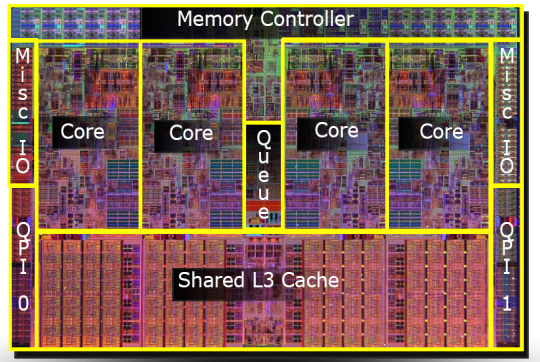
\includegraphics[height=1in]{images/nehalemdie}
    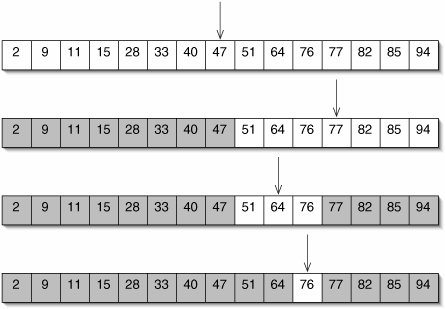
\includegraphics[height=1in]{images/binary-search}
    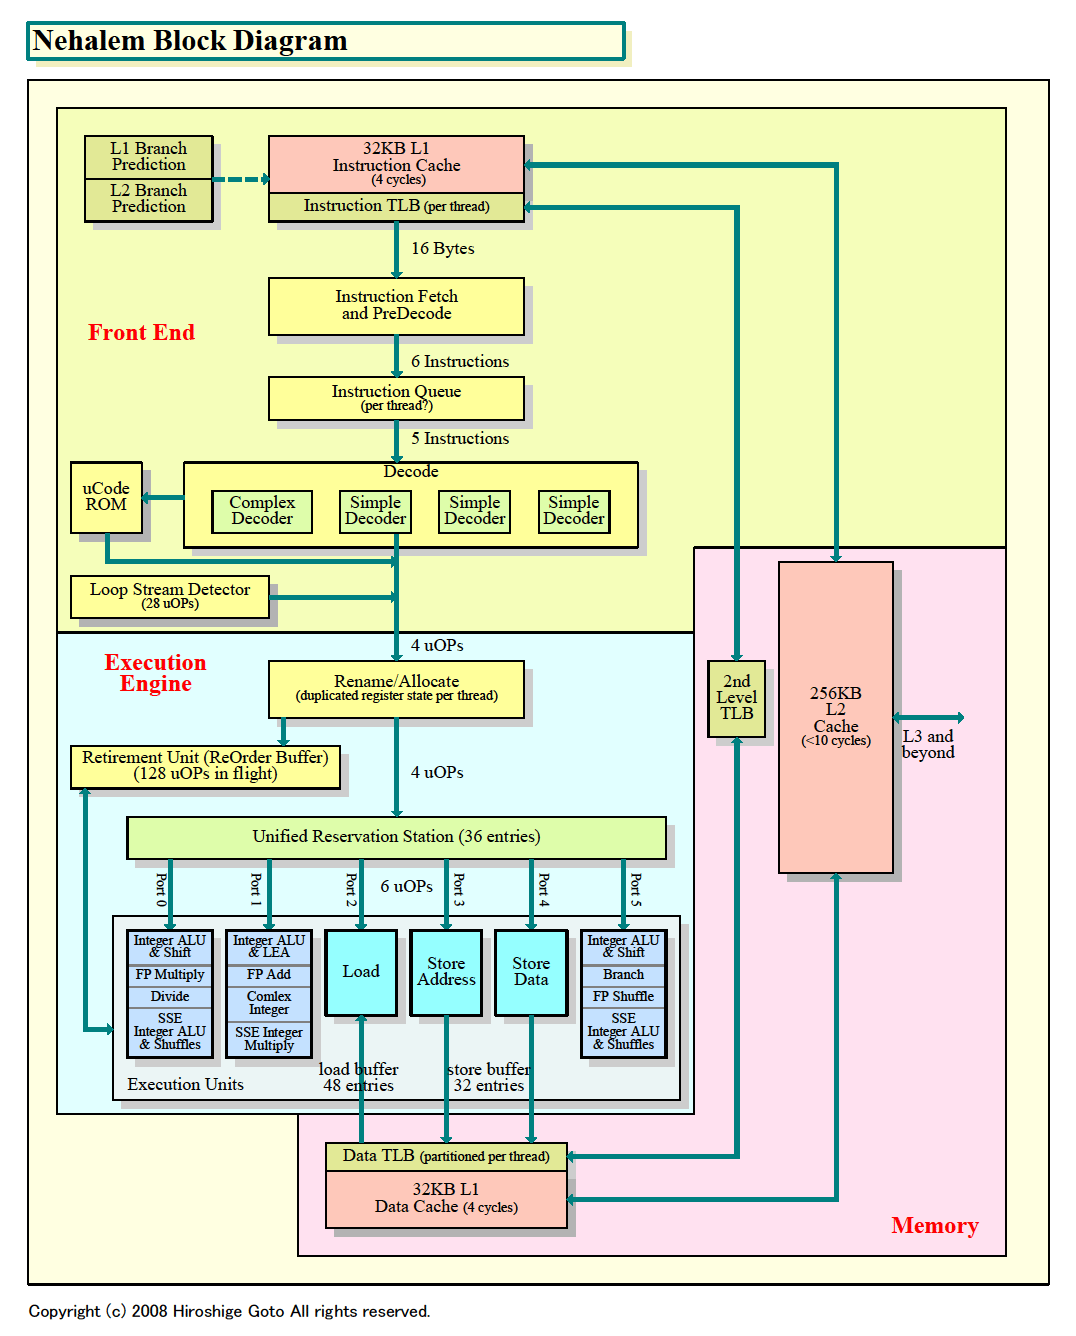
\includegraphics[height=1in]{images/nehalem-block}
  }
\end{frame}

\begin{frame}
  \frametitle{Microprocessor Architecture: Programmer's View}
  \framesubtitle{Von Neumann Architecture}

  \begin{center}
    \includegraphics[scale=0.85]{figs/programmers-view} 
  \end{center}
  
%  \begin{itemize}
%    \item<+->CPU repeatedly
%    \begin{itemize}
%      \item<+->Fetches an instruction (from RAM)
%      \item<+->Decodes the instruction
%      \item<+->Executes the instruction
%    \end{itemize}
%    \item<+->Instructions include:
%     \begin{itemize}
%      \item<+->Arithmetic operations on CPU registers
%      \item<+->Moving data between registers and RAM
%    \end{itemize}
%  \end{itemize}
  
\end{frame}


\begin{frame}
  \frametitle{Binary Search}
  \framesubtitle{The Classic Data Structure/Query Algorithm}

  \begin{center}
    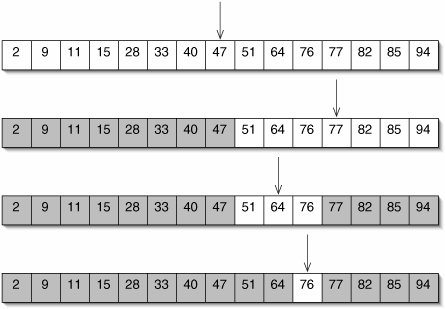
\includegraphics[width=.9\textwidth]{images/binary-search}
  \end{center}

\end{frame}


\begin{frame}[fragile]
  \frametitle{Binary Search}
  \framesubtitle{Branchy Code}

\begin{minted}{c++}
template<typename T, typename I>
I sorted_array<T,I>::branchy_search(T x) const {
    I lo = 0, hi = n;
    while (lo < hi) {
        I m = (lo + hi) / 2;
        if (x < a[m]) {
            hi = m;
        } else if (x > a[m]) {
            lo = m+1;
        } else {
            return m;
        }
    }
    return hi;
}
\end{minted}
\end{frame}

\begin{frame}[fragile]
  \frametitle{Binary Search: Analysis}

  \begin{itemize}
    \item<+->Each iteration of binary search either:
    \begin{itemize}
      \item<+->terminates (because \mintinline{c++}{x==a[m]})
      \item<+->terminates (because \mintinline{c++}{lo==hi})
      \item<+->Reduces \mintinline{c++}{hi-lo} by a factor of 2
    \end{itemize}
    \item<+->Binary search terminates after at most $\log_2 n$ iterations
    \item<+->Doubling the size of the array adds only one more iteration
  \end{itemize}
\end{frame}

\begin{frame}
  \frametitle{Binary Search: Experiments}
  \begin{center}
    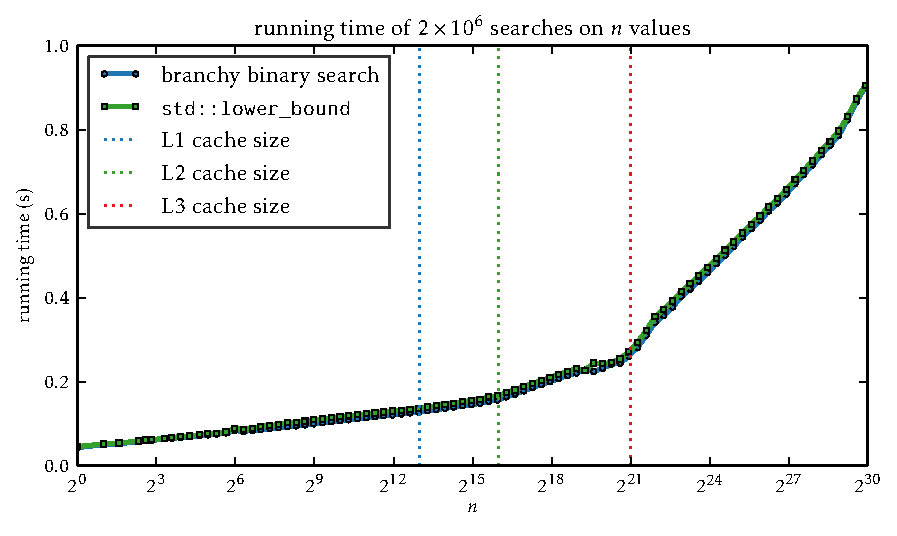
\includegraphics{graphs/sorted-i}
  \end{center}
\end{frame}

\begin{frame}[fragile]
  \frametitle{Binary Search}
  \framesubtitle{Branchy Assembly Code}

\vspace{-2em}
\footnotesize
%\resizebox{\textwidth}{\textheight}{
\begin{tabular}{p{.48\textwidth}p{.48\textwidth}}
\begin{minted}{nasm}
	.cfi_startproc
	movq	8(%rdi), %rax
	xorl	%ecx, %ecx
	movq	(%rdi), %r8
	cmpq	%rcx, %rax
	jbe	.L5
.L11:    ; top of while loop
	leaq	(%rcx,%rax), %rdx
	shrq	%rdx
	movl	(%r8,%rdx,4), %edi
	cmpl	%edi, %esi  ; a[m] <=> x
	jnb	.L3  ; jump if a[m] <= x
.L8:         ; a[m] > x
	cmpq	%rdx, %rcx
	movq	%rdx, %rax
	jnb	.L5
	addq	%rcx, %rdx
\end{minted} 
&
\begin{minted}{nasm}
	shrq	%rdx
	movl	(%r8,%rdx,4), %edi
	cmpl	%edi, %esi  ; x <=> a[m]
	jb	.L8
.L3:    ; a[m] <= x
	cmpl	%edi, %esi  ; x <=> a[m]
	jbe	.L7 ; jump if a[m] >= x
	leaq	1(%rdx), %rcx
	cmpq	%rcx, %rax
	ja	.L11
.L5:
	rep ret
.L7:
	movq	%rdx, %rax
	ret
	.cfi_endproc
\end{minted}
\end{tabular}
%}

\end{frame}

\begin{frame}
   \frametitle{The Instruction Pipeline}

   \begin{center}
      \multiinclude[<+>][start=1,format=pdf]{figs/pipeline}
   \end{center}
\end{frame}

\end{document}


\begin{frame}
  \frametitle{The Merge Sort Algorithm}

  \begin{tabular}{p{2.5in}p{1in}}
  \begin{itemize}
    \item<1->Used J. W. Bryce's Sorting maching in 1938 (U.S. Patent 2189024)
    \item<2->``Invented'' by John von Neumann in 1945
    \item<3->To sort #a[0]#\ldots #a[n-1]#:
    \begin{enumerate}
      \item<4-> sort #a[0]#\ldots #a[n/2]#
      \item<5-> sort #a[n/2+1]#\ldots #a[n-1]#
      \item<6-> merge the two sorted sequences
    \end{enumerate}
  \end{itemize}
  &
  \begin{center}
    \includegraphics[height=1.5in]{images/sorting}
  \end{center}
  \end{tabular}
\end{frame}


\begin{frame}

  \frametitle{Mergesort}
  \begin{itemize}
    \item<1->To sort #a[0]#\ldots #a[n-1]#:
    \begin{enumerate}
      \item<2-> sort #a[0]#\ldots #a[n/2]#  (recursively)
      \item<3-> sort #a[n/2+1]#\ldots #a[n-1]# (recursively)
      \item<4-> merge the two sorted sequences
    \end{enumerate}
    \item<1-> $\langle 9, 3, 5, 2, 1, 8, 7, 0, 6, 4 \rangle$
    \item<1->
     \only<1>{$\langle 9, 3, 5, 2, 1\rangle \langle 8, 7, 0, 6, 4 \rangle$}%
     \only<2>{$\langle 1, 2, 3, 5, 9\rangle \langle 8, 7, 0, 6, 4 \rangle$}
     \only<3>{$\langle 1, 2, 3, 5, 9\rangle \langle 0, 4, 6, 7, 8 \rangle$}
     \only<4>{$\langle 0, 1, 2, 3, 4, 5, 6, 7, 8, 9\rangle$}
  \end{itemize}
\end{frame}

\begin{frame}[fragile]
  \frametitle{Merging two sorted arrays}

  \begin{itemize}
    \item<1-> To merge two sorted arrays (or lists) #a# and #b# we scan them sequentially
  \end{itemize}
\begin{code}
  public <T extends Comparable<T>>
       void merge(T[] a, T[] b, T[] c) {
    int i = 0, j = 0, k = 0;
    while (i < a.length || j < b.length) {
      if (j == b.length) {
        c[k++] = a[i++];
      } else if (i == a.length) {
        c[k++] = b[j++];
      } else if (a[i].compareTo(b[j]) < 0) {
        c[k++] = a[i++];
      } else {
        c[k++] = b[j++];
      }
    }
  }
\end{code}
\end{frame}

\begin{frame}[fragile]
  \frametitle{Mergesort}

\begin{code}[fragile]
  public <T extends Comparable<T>>
      void mergeSort(T[] a) {
    if (a.length <= 1)
      return;
    T[] a1 = Arrays.copyOfRange
               (a, 0, a.length/2);
    T[] a2 = Arrays.copyOfRange
               (a, a.length/2, a.length);
    mergeSort(a1);
    mergeSort(a2);
    merge(a1, a2, a);
  }
\end{code}
\end{frame}

\begin{frame}
  \frametitle{Analysis of Mergesort}

  \begin{itemize}
    \item<1->Mergesort #a[0]#\ldots #a[n-1]#:
    \begin{enumerate}
      \item<2-> sort #a[0]#\ldots #a[n/2]#  (recursively)
      \item<3-> sort #a[n/2+1]#\ldots #a[n-1]# (recursively)
      \item<4-> merge the two sorted sequences
   \end{enumerate}
   \item<1-> Let $T(n)$ be the time to run merge sort on an array of length $n$
   \item<2-> Step 1 Takes $T(n/2)$ time
   \item<3-> Step 2 Takes $T(n/2)$ time
   \item<4-> Step 3 Takes $O(n)$ time
   \item<5-> $T(n) = O(n) + 2T(n/2)$\footnote{Cheating a bit here, assuming $n$ is a power of 2.}
  \end{itemize}
\end{frame}

\begin{frame}
  \frametitle{The Mergesort recurrence}

  \begin{itemize}
    \item<1-> $T(n) = O(n) + 2T(n/2)$
    \item<2->\only<2>{$T(n) = O(n) + 2O(n/2) + 4T(n/4)$}%
             \only<3->{$T(n) = O(n) + O(n) + 4T(n/4)$}%
    \item<4->\only<4>{$T(n) = O(n) + O(n) + 4O(n/4) + 8T(n/8)$}%
             \only<5->{$T(n) = O(n) + O(n) + O(n) + 8T(n/8)$}%
    \item<6->\only<6>{$T(n) = O(n) + O(n) + O(n) + \ldots nO(1)$}%
             \only<7->{$T(n) = O(n) + O(n) + O(n) + \ldots O(n)$}
    \item<8->$T(n) = O(n\log n)$
    \item<9->\textbf{Theorem:} The Mergesort algorithm can sort an array of $n$ items in $O(n\log n)$ time
  \end{itemize}
  TODO: Add figure 
\end{frame}

\begin{frame}
  \frametitle{Comparison-based sorting algorithms}

  \begin{itemize}
    \item<1-> So far, we have seen 3 sorting algorithms:
    \begin{itemize}
      \item<2-> Quicksort: $O(n\log n)$ expected time
      \item<3-> Heapsort: $O(n\log n)$ time
      \item<4-> Mergesort: $O(n\log n)$ time
    \end{itemize}
    \item<5-> Is there a faster (maybe $O(n)$ time) sorting algorithm?
    \begin{itemize}
      \item<6-> Answer: No and yes
    \end{itemize}
  \end{itemize}

\end{frame}

\begin{frame}
  \frametitle{Comparison-based sorting algorithms}

  \begin{itemize}
    \item<1-> Quicksort, Heapsort, and Mergesort are comparison-based
    \begin{itemize}
      \item<2-> All branching in the algorithm is based on the results
        of comparisons of the form #a[i] < b[i]#
      \item<3-> These algorithms can be used to sort any array of
        #Comparable# items
      \item<4-> But this comes at a price
      \begin{itemize}
        \item<5-> Every comparison-based sorting algorithm takes $\Omega(n\log n)$ time for some input
      \end{itemize}
    \end{itemize}
  \end{itemize}
\end{frame}


\begin{frame}
  \frametitle{Comparison trees}

  \begin{itemize}
    \item<1-> A \emph{comparison tree} is a full binary tree:
    \begin{itemize}
      \item<2-> each internal node #u# is labelled with a pair #u.i# and #u.j# 
      \item<3-> each leaf is labelled with a permutation of $\{0,\ldots,n-1\}$ 
    \end{itemize}
    \item<4-> For an array #a# we can \emph{run} the comparison tree   
    \begin{itemize}
      \item<5-> #u# is the root
      \item<6-> while #u# is not a leaf
      \begin{itemize}
        \item<7-> if $a[u.i] < a[u.j]$ then #u = u.left# else #u = u.right#
      \end{itemize}
    \end{itemize}
    \item<5-> The comparison tree \emph{sorts} if, for every input array #a#, the permutation at the leaf for #a# correctly sorts #a#
  \end{itemize}
  TODO: Add example of comparison tree for 3 elements
\end{frame}


\begin{frame}
  \frametitle{Comparison tree lower bound}
  
  \begin{itemize}
  \item<1->\textbf{Lemma:} Every comparison tree that sorts any input of length $n$ has at least $n!$ leaves
  \item<2->\textbf{Theorem:} Every comparison tree that sorts any input of length $n$ has depth at least $(n/2)\log_2 (n/2)$ 
  \begin{itemize}
    \item<3-> The height of a tree with $m$ leaves is at least $\log_2 m$
    \item<4-> The height of a tree with $n!$ leaves is at least $\log_2 n!$
    \item<5->[]
      
        \begin{eqnarray*} 
          \log_2 n!& =& \log_2(n) + \log_2(n-1) + \cdots+\log_2(1) \\
                   &\ge&\log_2(n) + \cdots+\log_2(n/2) \\
                   &\ge&\log_2(n/2) +\cdots+\log_2(n/2) \\
                   &=&(n/2)\log_2(n/2)
        \end{eqnarray*}
   \end{itemize}
  \end{itemize}
\end{frame}

\begin{frame}
  \frametitle{Comparison-based sorting and comparison trees}

  \begin{itemize}
    \item<1->Every deterministic comparison-based sorting algorithm $\mathcal{A}$ that can sort every array of $n$ elements defines a comparison tree $T_\mathcal{A}$ that sorts
    \item<1->TODO: Show relationship between SelectionSort and comparison tree
    \item<2->The height of $T_\mathcal{A}$ is equal to the (worst-case) number of comparisons that $\mathcal{A}$ performs
    \item<3->\textbf{Theorem:} For every deterministic comparison-based sorting algorithm $\mathcal{A}$, there exists an input such that $\mathcal{A}$ requires $\Omega(n\log n)$ comparisons
  \end{itemize}
  TODO: Discuss randomized algorithms
\end{frame}

\begin{frame}
  \frametitle{Summary}

  \begin{itemize}
    \item<1-> Mergesort: runs in $O(n\log n)$ time
    \item<2-> Any comparison-based sorting algorithm requires $\Omega(n\log n)$ time
    \item<3-> Mergesort, Quicksort, and Heapsort are optimal comparison-based sorting algorithms
    \item<4-> In-class problem:
    \begin{itemize}
      \item<5-> Design an algorithm that takes an array #a# of #n# integers in the range $\{0,\ldots,n-1\}$ and sorts them in $O(n)$ time
    \end{itemize}
  \end{itemize}
\end{frame}
\end{document}

\begin{frame}
  \frametitle{Priority queues}
  \begin{itemize}
    \item<1->A \emph{priority queue} stores a collection of #Comparable# elements
    \item<2->Operations:
    \begin{itemize}
      \item<3-> #add(x)# : Add #x# to the collection
      \item<4-> #findMin()# : Return the smallest element in the collection
      \item<5-> #deleteMin()# : Remove the smallest element in the collection
    \end{itemize}
    \item<6-> In the JCF Queue interface, these are:
    \begin{itemize}
      \item #add(x)/offer(x)# : #add(x)#
      \item #peek()# : #findMind()#
      \item #remove()/poll()# : #deleteMin()#
    \end{itemize}
  \end{itemize}
\end{frame}

\begin{frame}[fragile]
  \frametitle{Application 1: Sorting}

  \begin{itemize}
    \item We can sort a set of elements by inserting them all into a priority queue and then removing them  
  \end{itemize}
\begin{code}
  public static <T> void sort(T[] a) {
    Queue<T> pq = new PriorityQueue<T>();
    for (T x : a) 
      pq.add(x);
    for (int i = 0; i < a.length; i++)
      a[i] = pq.remove();
  }
\end{code}
\end{frame}

\begin{frame}[fragile]
  \frametitle{Application 2: Queueing systems}

\begin{code}
class Packet implements Comparable<Packet> {
  int compareTo(Packet p) {
    return this.priority - p.priority;
  }
  ...
}
class NetworkSwitch {
  public void receive(Packet p) {
    pq.add(p);
  }
  ...
  public void sendNext() {
    send(pq.remove());
  }
}
\end{code}
\end{frame}

\begin{frame}
  \frametitle{Application 3: Simulation}
 
  \begin{itemize}
    \item<1->In simulations, priority queues store events ordered by time of occurrence
  \end{itemize}
  \multiinclude[<+>][start=1,format=pdf,width=3in]{figs/sim}
\end{frame}

\begin{frame}
  \frametitle{Heaps}
  \begin{itemize}
    \item<1-> Priority queues can be implemented as (binary) \emph{heaps}
    \item<2-> A binary heap is a binary tree where each node #u# stores a value #u.prio#
    \begin{itemize}
      \item<3-> Heap property: #u.prio < u.left.prio# and #u.prio < u.right.prio#
    \end{itemize}
  \end{itemize}
  \begin{center}
    \includegraphics{figs/heap}
  \end{center}
\end{frame} 


\begin{frame}
  \frametitle{Complete binary heaps}
  \begin{itemize}
    \item<1-> A \emph{complete} heap uses a complete binary tree:
    \begin{itemize}
      \item<2->A complete binary tree of height $d$ has up to $2^{d+1}-1$ nodes
      \item<3->To store $n$ nodes, we require $2^{d+1}-1 \ge n$
      \begin{itemize}
        \item<4->$2^{d+1} \ge n+1$
        \item<5->$d+1 \ge \log_2(n+1)$
        \item<6->$d \ge \log_2(n+1)-1\only<7->{= O(\log n)}$
      \end{itemize}
      \item[] \begin{center}\includegraphics[width=2.5in]{figs/heap}\end{center}
    \end{itemize}
    \item<7-> A complete heap of size $n$ has height $O(\log n)$
  \end{itemize}
  \end{frame} 


\begin{frame}
  \frametitle{Ahnentafel lists}
 
  \begin{itemize}
    \item<1->The \emph{Eytzinger method} maps the nodes of a complete binary tree to the positions of an array #a#
    \begin{itemize}
      \item<2-> #a[0]# is the root
      \item<3-> the left child of #a[i]# is #a[2*i+1]#
      \item<4-> the right child of #a[i]# is #a[2*i+2]#
      \item<5-> the parent #a[i]# is #a[(i-1)/2]#
    \end{itemize}
    \item[]\begin{center}\begin{tabular}{cc}
             \includegraphics[height=1.2in]{figs/ahnentafel}&
             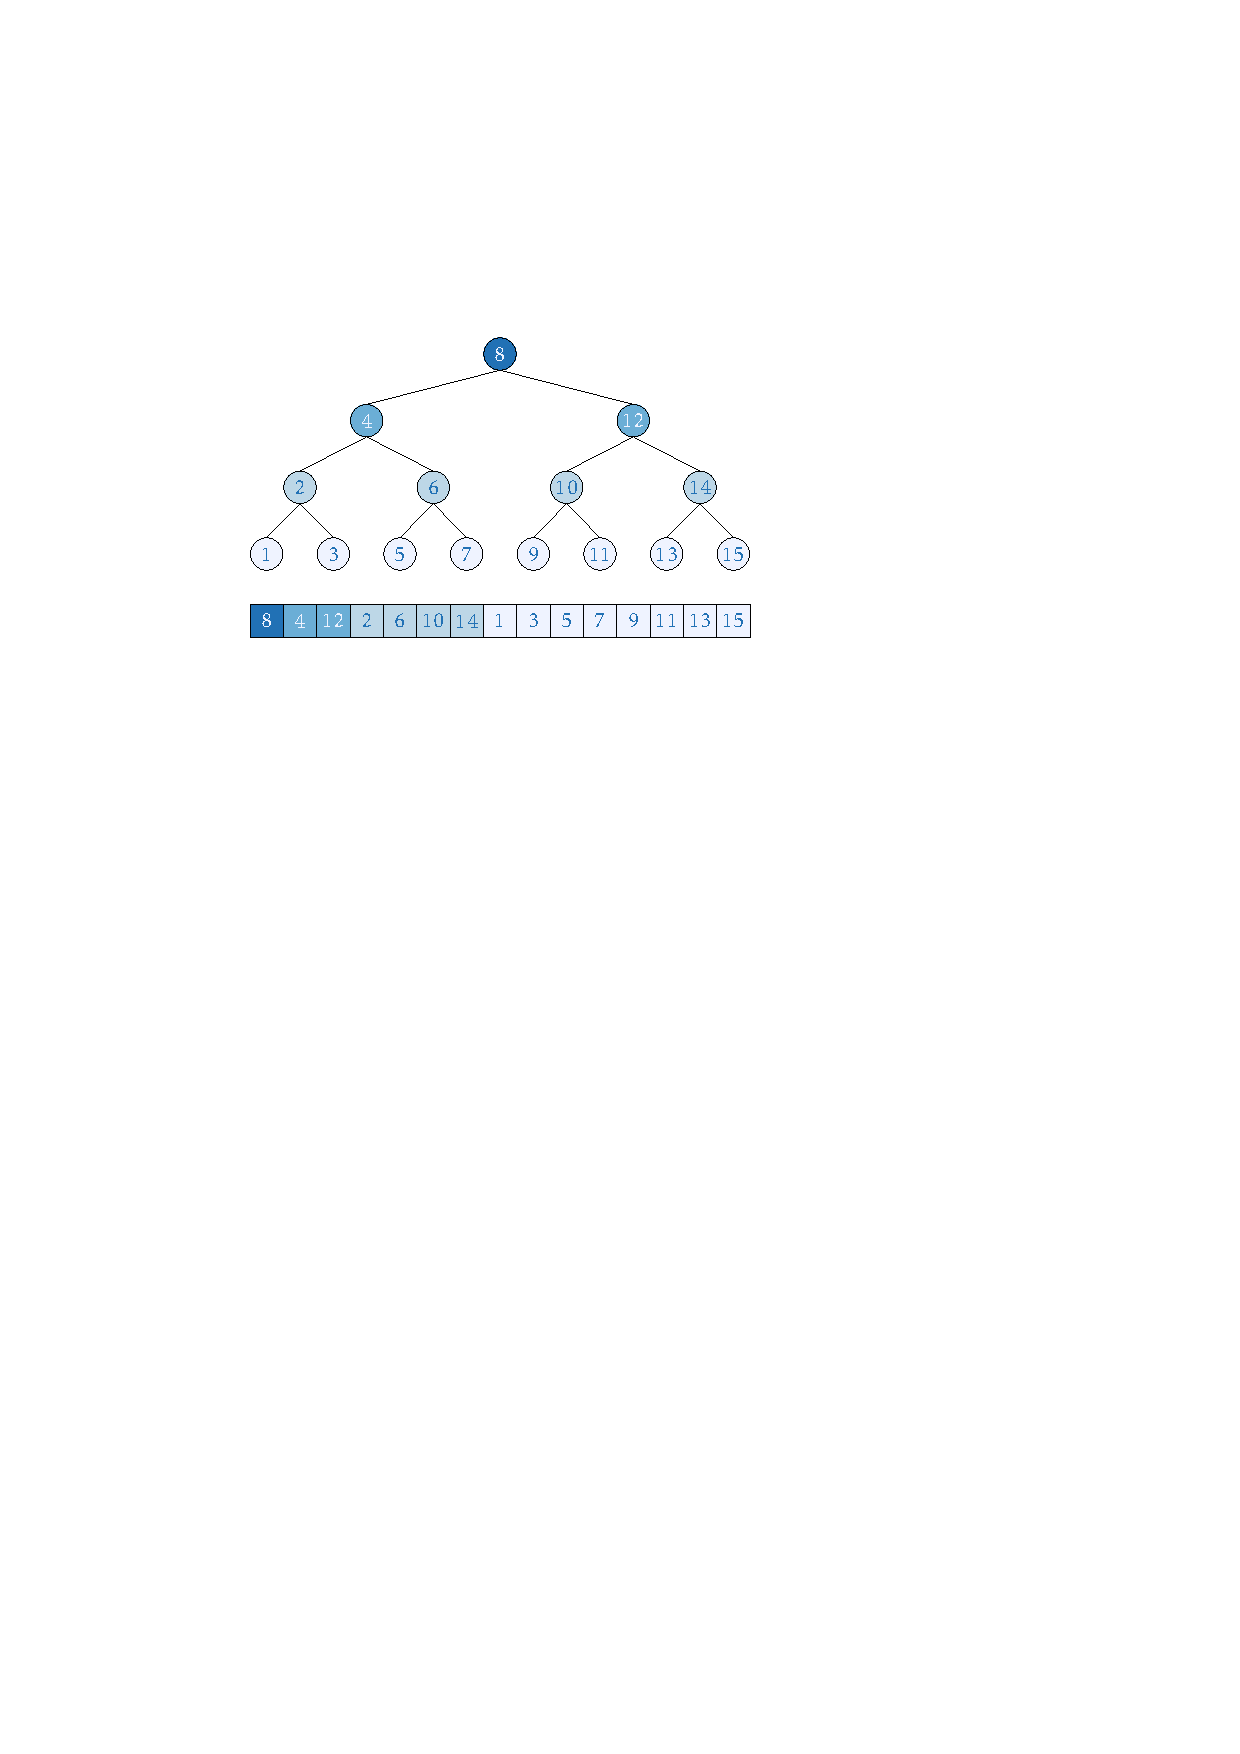
\includegraphics[height=1.2in]{images/eytzinger}
           \end{tabular}\end{center}
  \end{itemize}
\end{frame}

\begin{frame}[fragile]
  \frametitle{Implicit binary heaps}

  \begin{itemize}
    \item<1->An \emph{implicit binary heap} represents a complete binary heap in an array #a# using the Eytzinger method
    \item<2->[]\begin{center}\includegraphics[width=2.5in]{figs/binheap}\end{center}
    \item<3-> No extra pointers, all the data lives in #a#
  \end{itemize}
\end{frame} 


\begin{frame}[fragile]
\begin{code}
public class BinaryHeap<T extends Comparable<T>>
      extends AbstractQueue<T> {
  protected T[] a;
  protected int n;

  protected int left(int i) {
    return 2*i + 1;
  }

  protected int right(int i) {
    return 2*i + 2;
  }

  protected int parent(int i) {
    return (i-1)/2;
  }
  ...
}
\end{code}
\end{frame}

\begin{frame}[fragile]
  \frametitle{Finding the min}

  \begin{itemize}
    \item<1->Finding the minimum value in a heap is easy
    \begin{itemize}
      \item<2->It's stored at the root
      \item<3->This is #a[0]#
    \end{itemize}
    \item<4->[]
\begin{code}
  public T peek() {
    return a[0];
  }
\end{code}
    \item<5->Runs in $O(1)$ time
  \end{itemize}
\end{frame}

\begin{frame}
  \frametitle{Inserting into a heap}

  \begin{itemize}
    \item<1->To insert #x# into a (implicit binary) heap, we
    \begin{enumerate}
      \item<2->add #x# as a leaf
      \item<3->while #x# is smaller than #parent(x)#
      \begin{itemize}
        \item<4-> swap #x# with its parent
      \end{itemize}

    \end{enumerate}
    \item[]\begin{center}
      \includegraphics[width=2.5in]{figs/binheap}
    \end{center}
    \item<5->Runs in $O(\log n)$ time
  \end{itemize}
\end{frame} 


\begin{frame}[fragile]
\begin{code}
  public boolean offer(T x) {
    if (n + 1 > a.length)
      grow();
    a[n++] = x;
    bubbleUp(n-1);
    return true;
  }
  protected void bubbleUp(int i) {
    int p = parent(i);
    while (i > 0 && a[i].compareTo(a[p]) < 0) {
      swap(i,p);
      i = p;
      p = parent(i);
    }
  }
\end{code}
\end{frame}


\begin{frame}
  \frametitle{Deleting from a heap}
  \begin{itemize}
    \item<1->To delete the min from a heap, we
    \begin{enumerate}
      \item<2->copy #x=a[n-1]# into #a[0]#
      \item<3->while #x# is larger than either of its children
      \begin{itemize}
        \item<4-> swap #x# with the smaller of its children
      \end{itemize}
    \end{enumerate}
    \item[]\begin{center}
      \includegraphics[width=2.5in]{figs/binheap}
    \end{center}
    \item<5->Runs in $O(\log n)$ time
  \end{itemize}
\end{frame}

\begin{frame}[fragile]
\begin{code}
  public T poll() {
    T x = a[0];
    swap(0, --n);
    trickleDown(0);
    return x;
  }
\end{code}
\end{frame}

\begin{frame}[fragile]
\begin{code}
  protected void trickleDown(int i) {
    do {
      int j = -1;
      int r = right(i);
      if (r < n && a[r].compareTo(a[i]) < 0) {
        int l = left(i);
        if (a[l].compareTo(a[r]) < 0) {
          j = l;
        } else {
          j = r;
        }
      } else {
        int l = left(i);
        if (l < n && a[l].compareTo(a[i]) < 0) {
          j = l;
        }
      }
      if (j >= 0)  swap(i, j);
      i = j;
    } while (i >= 0);
  }
\end{code}
\end{frame}

\begin{frame}
  \frametitle{Summary so far}

  \begin{itemize}
    \item \textbf{Theorem:} A (implicit) binary heap supports the operations #add(x)# and #deleteMin()# in $O(\log n)$ (amortized) time and supports the #findMin()# operation in $O(1)$ time.
  \end{itemize} 
\end{frame}

\begin{frame}[fragile]
  \frametitle{Building a heap}
 
  \begin{itemize}
    \item<1-> Suppose we are given an unsorted array #a#
    \item<2-> How quickly can we make #a# into an implicit binary heap?
    \item<3-> #a[0]# How quickly can we make #a# into an implicit binary heap?
    \item<4-> We can insert elements #a[0],...,a[n-1]# one at a time
\begin{code}
  public BinaryHeap(T[] ia) {
    a = ia;
    for (int n = 1; n < a.length; n++) {
      add(a[n]);
    }
  }
\end{code}
    \item<5-> This takes $O(1+\log(1)) + O(1+\log(2)) + \cdots O(1+\log n)$ time
    \item<6-> ${}= O(n\log n)$
    \item<7-> Can we do better?
  \end{itemize}
\end{frame}


\begin{frame}[fragile]
  \frametitle{Building a heap in linear time}
 
  \begin{itemize}
    \item<1-> We can do better by working bottom up
    \item<2-> First build $\approx n/2$ heaps of size 1
    \item<3-> Next, build $\approx n/4$ heaps of size 3
    \item<4-> Next, build $\approx n/8$ heaps of size 7
    \item<5-> \ldots
    \item<6-> Build $1$ heap of size $n$
    \item<7->[]
\begin{code}
  public BinaryHeap(T[] ia) {
    a = ia;
    n = a.length;
    for (int i = n/2; i >= 0; i--) {
      trickleDown(i);
    }
  }
\end{code}
  \end{itemize}
\end{frame}

\begin{frame}
  \frametitle{Building a heap in linear time - analysis}

  \begin{itemize}
    \item<1-> We call #trickleDown(i)# $n/2^{j}$ times where $j$ is the root of heap of size $2^j-1$
    \item<2-> #trickleDown(i)# then takes $O(\log (2^j-1)) = O(j)$ time
    \item<3-> Total running time is
    \begin{itemize}
      \item<4->$(n/4)\cdot O(1)$
      \item<5->$(n/8)\cdot O(2)$
      \item<6->$(n/16)\cdot O(3)$
      \item<7->\ldots
      \item<8->$1\cdot O(\log n)$
      \item<9->${} = O(n)$\footnote{COMP3804 exercise}
    \end{itemize}
  \end{itemize}
\end{frame}


\begin{frame}[fragile]
  \frametitle{Heapsort}

  \begin{itemize}
    \item<1->The heapsort algorithm for sorting an array #a# of length $n$:
    \item<2->Make #a# into a heap in ($O(n)$ time)
    \item<3->Repeat $n$ times:
    \begin{itemize}
      \item<4->Delete the minimum
    \end{itemize}
    \item<5->[]
\begin{code}
public T deleteMin() {
    swap(0, --n);
    trickleDown(0);
  }
\end{code}
    \item<6->Each deletion takes $O(\log n)$ time
    \item<7->Runs in $O(n\log n)$ time
    \item<8->Doesn't require any extra space --- does all work inside of input array #a#
  \end{itemize}
\end{frame}

\end{document}

